آ)\\
به صورت تمیز تر می توان دستورات را به صورت ترتیبی نوشت\\
\begin{latin}
while(R1 != 0)\{\\
\quad R2 = R2 \% R1;\\
\quad R2 = R1 xor R2;\\
\quad R1 = R1 xor R2;\\
\quad R2 = R1 xor R2;\\
\}\\
\end{latin}
سه 
xor
ای که بعد مد گیری آمده است در واقع 
$R2$
را با
$R1$
جابجا می کند.
خط اول نیز باقی مانده میگیرد.
در واقع این پیاده سازی الگوریتم اقلیدس برای پیدا کردن ب.م.م است.
این مقادیر به این صورت تغییر می کند.\\
\begin{latin}
$R0 = 0, R1 = 36, R2 = 27$\\
$R0 = 1, R1 = 36, R2 = 27$\\
$R0 = 2, R1 = 36, R2 = 63$\\
$R0 = 3, R1 = 27, R2 = 63$\\
$R0 = 4, R1 = 27, R2 = 36$\\
$R0 = 0, R1 = 27, R2 = 36$\\
$R0 = 1, R1 = 27, R2 = 9$\\
$R0 = 2, R1 = 27, R2 = 18$\\
$R0 = 3, R1 = 9, R2 = 18$\\
$R0 = 4, R1 = 9, R2 = 27$\\
$R0 = 0, R1 = 9, R2 = 27$\\
$R0 = 1, R1 = 9, R2 = 0$\\
$R0 = 2, R1 = 9, R2 = 9$\\
$R0 = 3, R1 = 0, R2 = 9$\\
\end{latin}
ب)
\begin{center}
    
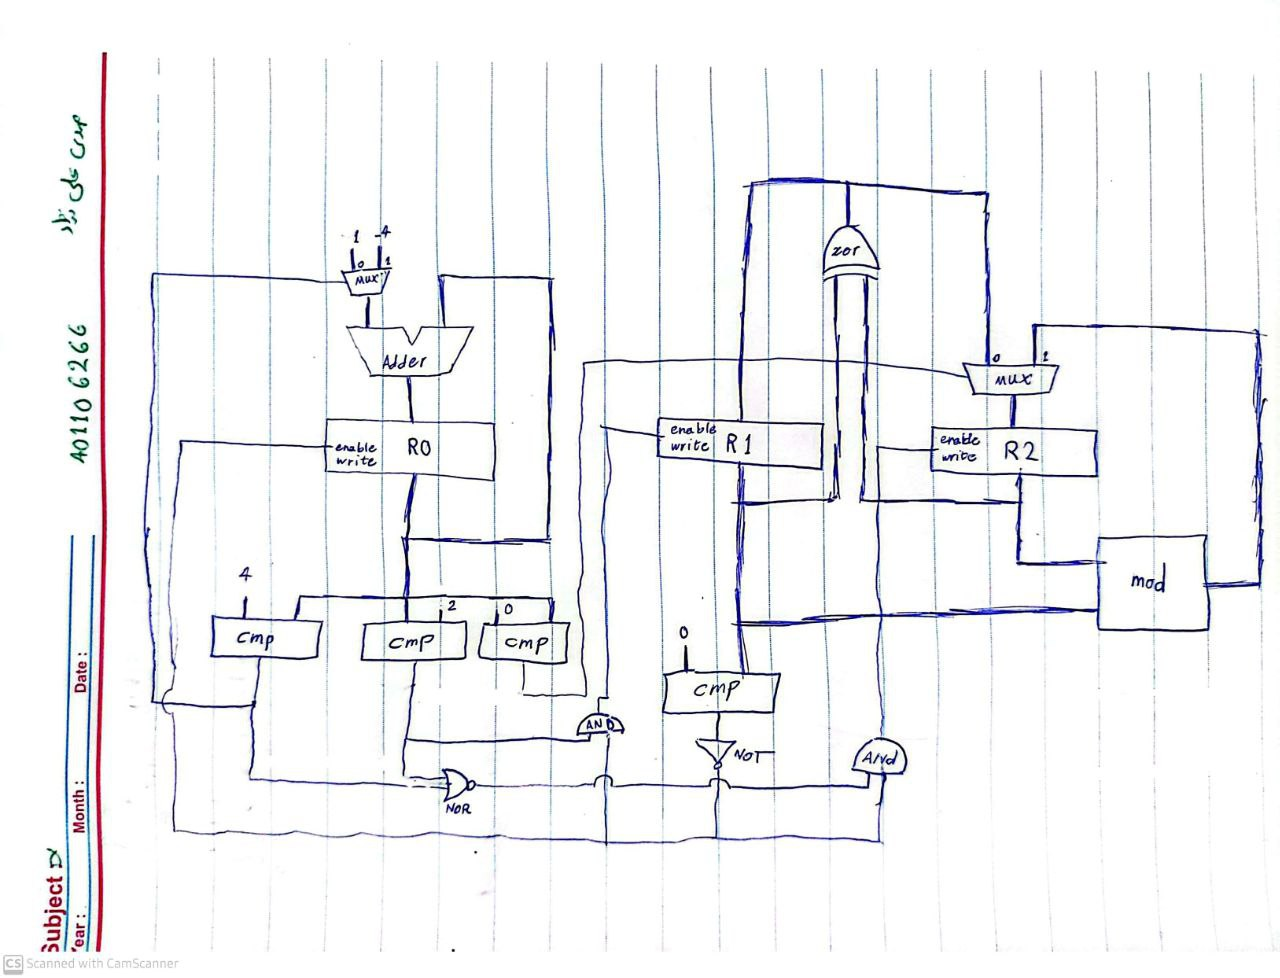
\includegraphics[width=\textwidth]{images/shematic2.png}
\end{center}